\documentclass [a4paper,12 pt]{article}
\usepackage{times}
\usepackage{tabu}
\usepackage{a4,color,palatino,amsmath,amsthm,natbib,amssymb,graphicx,setspace}
\usepackage{fullpage}
\usepackage[multiple]{footmisc}
\usepackage{tikz}
\usepackage{wrapfig}
\usepackage{natbib}
\usepackage{url}
\usepackage{lipsum}
\newtheorem{prop}{Proposition}
\newtheorem{ass}{Assumption}
\newtheorem{cor}{Corollary}
\newtheorem{res}{Result}
\newtheorem{rem}{Remark}
\newtheorem{conj}{Conjecture}
\newtheorem{lem}{Lemma}
\DeclareMathOperator*{\argmin}{arg\,min}
\DeclareMathOperator*{\argmax}{arg\,max}
\setcounter{secnumdepth}{1}





\pdfinfo{
   /Title  (Predicting crime levels with machine learning)
	
}

\newenvironment{mfignotes}{\begin{footnotesize}\begin{minipage}{\textwidth}\begin{footnotesize}\smallskip\par}
{\end{footnotesize}\end{minipage}\end{footnotesize}}


\linespread{1.5}

\begin{document}


\title{Predicting crime levels in Washington DC with machine learning}
\title{CEGEG076 \\ 
Spatio-Temporal Data Mining \\ 
\vspace{15mm}
Prediction of crime levels in Washington DC, based on seasonality and census data}
\maketitle

\section*{Summary}
In this paper, we critically assess the performance of methods of machine-learning with the aim of predicting areas of high and low seasonal burglary rates in Washington, DC. We present two techniques: Random Forest (RF) and Support Vector Machine (SVM). It is generally agreed that Random Forest and SVM are amongst the best performing classifiers, and both have been used effectively in crime classification. Random Forest and Support Vector Machines both take a set of classified training data and output predicted classifications for another set of input variables. In our experiment, SVM performed better than Random Forest by only a small margin which is likely not statistically significant. However, Random Forest proved to be a better performer in terms of ease of implementation, speed, and interpretability.


\vspace{10mm}
\subsubsection*{Word count : XXXX}
\vspace{10mm}
\subsubsection*{Authors: Duccio Aiazzi, Sarah Hank}

\clearpage

\tableofcontents{}

\clearpage











\section{Introduction}
%%%%%%%%%%%%%%%%%%%%%%%%%%%%%% INTRODUCTION
This experiment aims to compare the use of two classification algorithms to predict levels of crime in Washington, DC: Support Vector Machines (SVM) \citep{vapnik1974theory} and Random Forest \citep{breiman2001random}. We use various demographic, economic, and housing factors to classify census tracts into either high or low crime categories. Though the first idea was to develop a model to predict crime at a very fine temporal scale using variables easy to monitor on a daily basis, the project later turned to a model to predict crime levels from one year to the other using census data. Therefore, the scope of the model changed from a daily prediction to a resource allocation tool on a yearly or seasonal basis.


\section{Methods}\label{methods}
We chose to use SVM and Random Forest as they rank very high in terms of classifier performances \citep{fernandez2014we} and because we are interested in spotting the interaction of crime with other measurable variables. Of course other methods would have been appropriate too: for example, given that crime is spatially and temporally autocorrelated \citep{anselin2000spatial}, a Space Time AutoRegressive Integrated Moving Average (STARIMA) or Space Time Scan Statistics (STSS) model would have been effective in spotting hotspots and patterns \citep{olligschlaeger1997spatio}. However, these methods are limited to space and time factors and do not take into account other variables. 
 
The use of Random Forest as a predictor for crime is relatively new, and thus there is not a large amount of literature exploring its effectiveness. The literature that does exist, however, seems to tout the method's success. \cite{bogomolov2014once} compared methods of ANN, SVM, and Random Forest using human behavior from aggregated mobile data in addition to demographic factors to predict crime hotspots in London \citep{bogomolov2014once}. They concluded that Random Forest was the most successful of these methods, with a successful prediction rate of 70\%. Another study by \cite{breitenbachcreating} compared random forests, support vector machines, gradient descent, neural networks, and ADTree, as well as logistic regression methods to predict violent arrests after prison release and also found Random Forest to perform the best. Because SVM methods have been proposed much longer ago, more literature is available on crime prediction. As a classifier, it is mainly used in finding hotspots, or areas with relatively higher rates of crime. \cite{kianmehr2008effectiveness} compare the success of one-class and two-class SVMs against neural networks and Structure Activity Relationships (SAR) in classifying crime hotspots in Columbus, Ohio and St. Louis, Missouri, and find that two-class SVMs work the best.

\section{Data}\label{sec_data}
%%%%%%%%%%%%%%%%%%%%%%%%%%%%%%% DATA

The crime data we investigate comes from the District of Columbia's Metropolitan Police Department's Crime Map tool \citep{metPolice}. The data contains crimes related to theft, robbery, and burglary and other violent crimes. Each incident comes with associated date and time of occurrence, the type of crime (offense), and the location of the crime presented as latitude and longitude, as well as the census tract in which it occurred. We use census tracts as our areal unit of analysis since this gives us the ability to analyze census data which is also aggregated by census tract. 

As mentioned earlier, we originally intended to use weather data as a variable to try to partially predict crime rate variations on an almost daily basis. The idea came from the literature review: the link between crime and weather is well-documented, and generally concludes that warmer temperatures result in more crime, specifically crimes of aggression \citep{cohn1990weather}. When we looked at our data, though, we did not find any correlation. In fact, there is a clear seasonal pattern in the count of crimes and therefore a correlation between this and temperature. We normalised temperature in two ways: first by taking the absolute deviation from the 30 year historical average for that day, and second by calculating a Z-score for that day's average temperature relative to the average temperatures from the preceding 14 days. Once we eliminated the seasonality by normalising the temperature, we found that relative variation in temperature has no correlation at all with crime rates. Therefore we decided to move our attention to a longer term prediction based on census data.

%income 
\begin{figure}[h!]
\begin{center}
\begin{tabular}{cc}
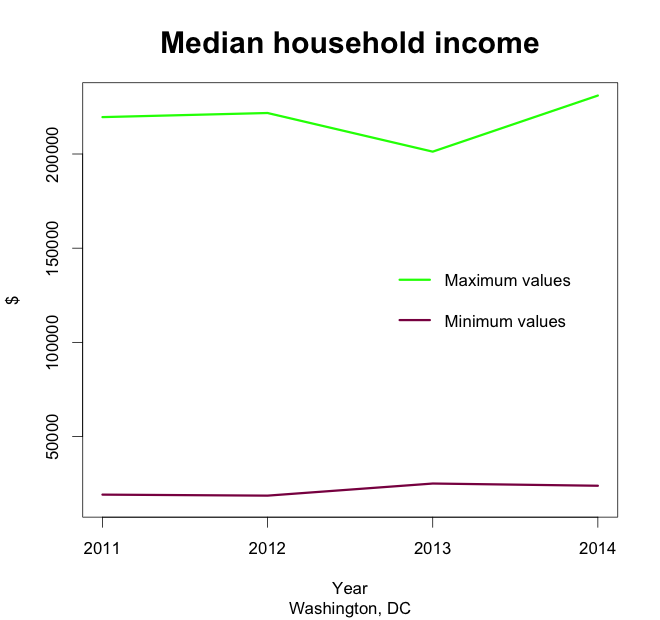
\includegraphics[viewport=5 0 660 600,clip,scale=0.33]{Figures/EDA_income.png}&
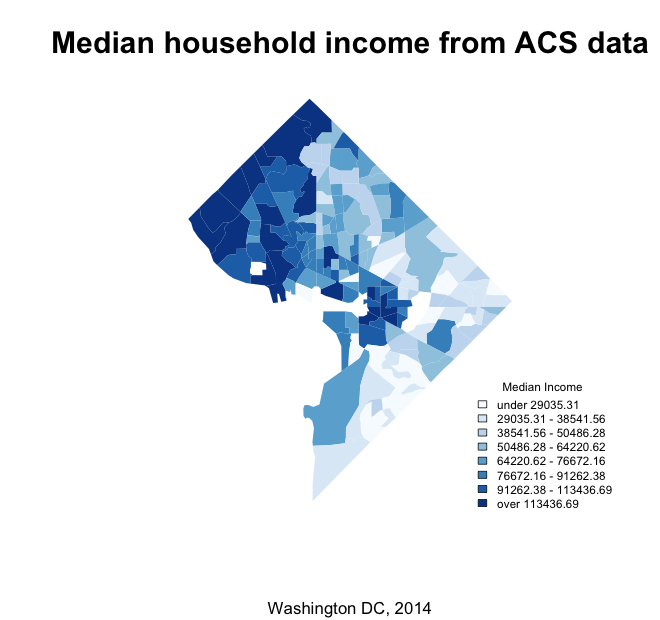
\includegraphics[viewport=10 0 660 600,clip,scale=0.33]{Figures/EDA_income_m.png}
\end{tabular}
\caption{Levels of income}\label{EDA_income}				
\scalebox{1}{
\begin{mfignotes}
Map indicates clear segregation between wealthy and deprived areas.
\end{mfignotes}
}
\end{center}
\end{figure}

Violent crime crime is, of course, associated with deprived conditions and there is a vast body of  literature on the subject: \cite{ehrlich1975relation} on the relation with educational attainment, \cite{ellis2009handbook} on unemployment, \cite{patterson1991poverty} on income and deprivation. For our study, we extracted a set of indicators from the American Community Survey 5 year-estimates for each year from 2011 - 2014. The indicators are related to household types, educational attainment, unemployment levels, income, house occupancy, house values, and age classes. For the full list of variables see Table \ref{table:variables} in Section \ref{appendix}. Our goal is to spot non-linear dynamics amongst these variables and the rates of crime per area. One example could be the subject of age class: it is reasonable to expect more burglaries committed by younger persons. However, offenders do not necessarily commit crimes in the places where they live, but rather might chose to commit their crime in a residential area with higher housing value or income level. Therefore, crime patterns will likely interact with income data both in terms of where offenders are and where they commit a crime.


Below is a visualization of the data from four of the census input variables: Median Income, Poverty Level, Median Age, and Unemployment Level. Each map visualizes the data for the year 2014, while each line chart shows the change over the four years for the tracts with the highest and lowest values. These graphs provide context in both the variability of the data as well as the landscape of the city.

%povLev
\begin{figure}[h!]
\begin{center}
\begin{tabular}{cc}
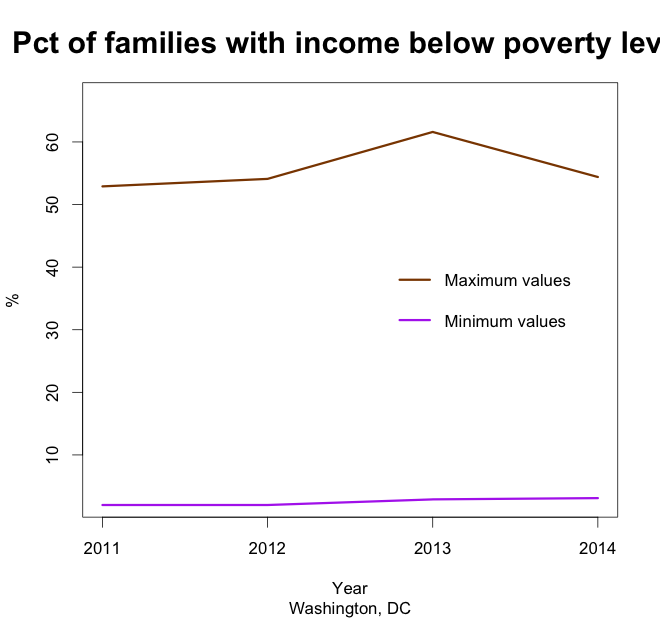
\includegraphics[viewport=5 0 660 600,clip,scale=0.33]{Figures/EDA_povLev.png}&
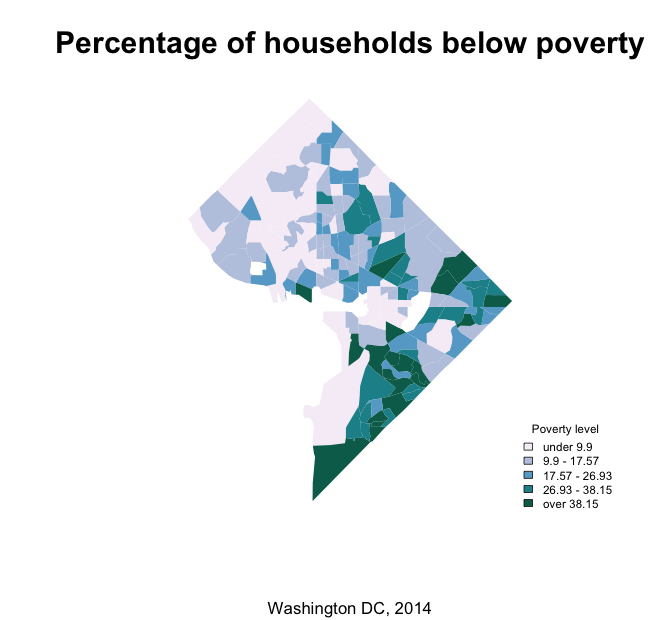
\includegraphics[viewport=10 0 660 600,clip,scale=0.33]{Figures/EDA_povLev_m.png}
\end{tabular}
\caption{Percentage of family below poverty levels}\label{EDA_povLev}				
\scalebox{1}{
\begin{mfignotes}
Concentration of poverty is mostly seen in southern part of the city.
\end{mfignotes}
}
\end{center}
\end{figure}



The map of median income (Fig. \ref{EDA_income}, page \pageref{EDA_income}) clearly displays a key feature of the landscape of DC: inequality. Tracts west of 16th St (the road which divides DC from the top point of the diamond) and tracts around Capitol Hill (the chunk of darker tracts in the Eastern part of the city) are fairly distinctly separated from poorer tracts. The max and min tracts show little variability over time except a slight dip in the values of the max tract in 2013. 

%Age
\begin{figure}[h!]
\begin{center}
\begin{tabular}{cc}
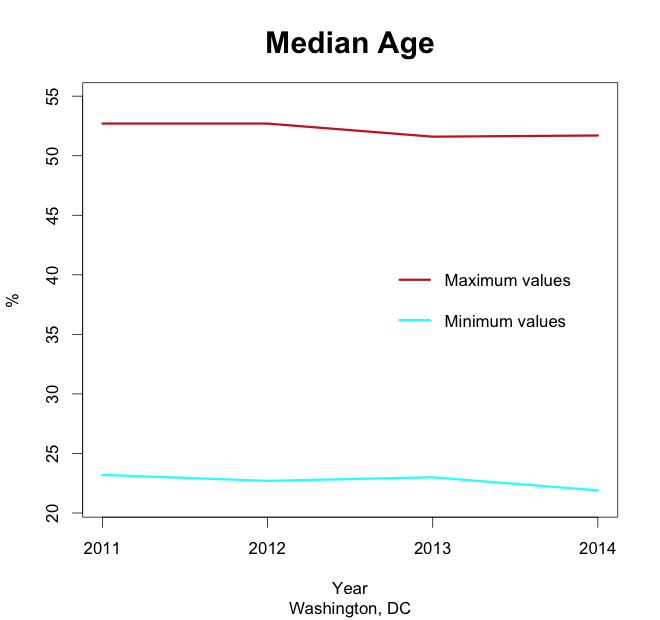
\includegraphics[viewport=5 0 660 600,clip,scale=0.33]{Figures/EDA_age.png}&
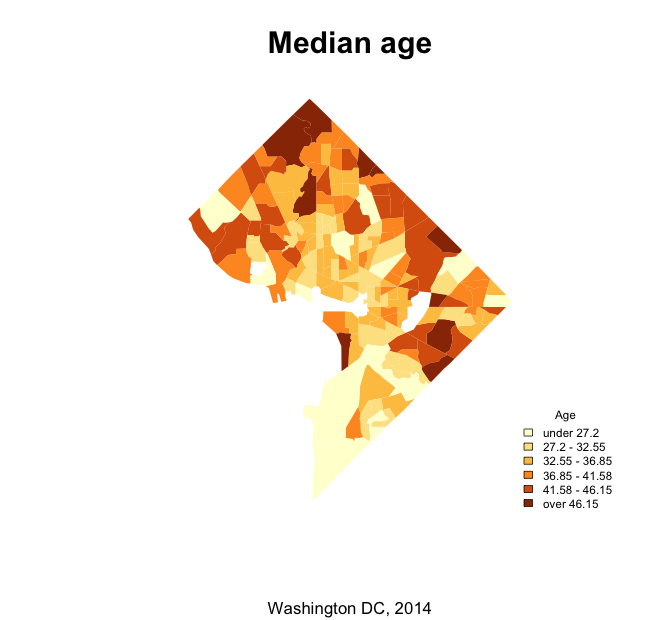
\includegraphics[viewport=10 0 660 600,clip,scale=0.33]{Figures/EDA_age_m.png}
\end{tabular}
\caption{Median age}\label{EDA_age}				
\scalebox{1}{
\begin{mfignotes}
Median age is highly variable across the city.
\end{mfignotes}
}
\end{center}
\end{figure}




The map in Fig. \ref{EDA_povLev} (page \pageref{EDA_povLev}) shows high spatial clustering of high poverty tracts in the south and south east, the poorest part of the city. Some of the darker tracts in the north west quadrant contain college campuses. The min tract changes very little over time, which is expected since the wealthier parts of the city will tend to stay wealthy. The max tract varies between 50\% and 60\%, mirroring the trend in unemployment.

%Unemployment
\begin{figure}[h!]
\begin{center}
\begin{tabular}{cc}
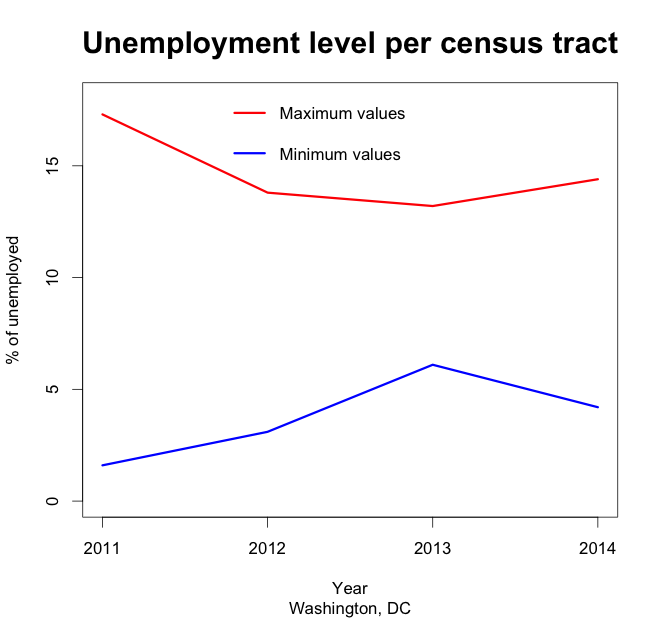
\includegraphics[viewport=5 0 660 600,clip,scale=0.33]{Figures/EDA_unempl.png}&
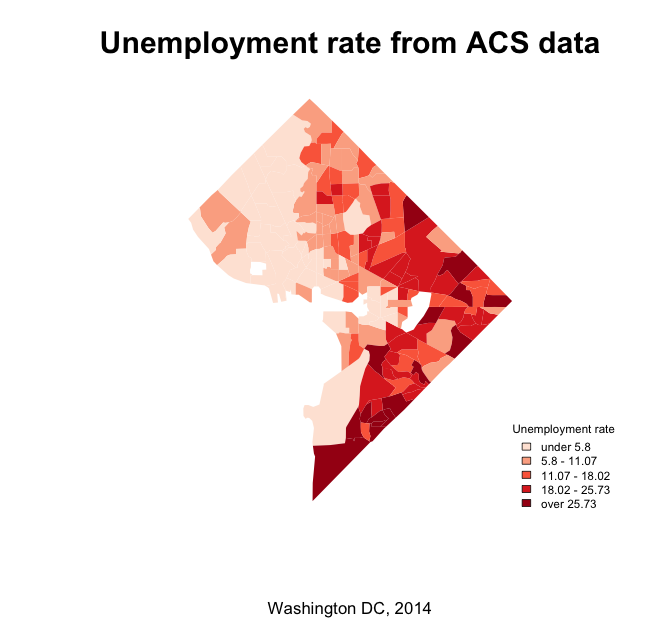
\includegraphics[viewport=10 0 660 600,clip,scale=0.33]{Figures/EDA_unempl_m.png}
\end{tabular}
\caption{Unemployment rate}\label{EDA_unempl}				
\scalebox{1}{
\begin{mfignotes}
Unemployment levels mirror segregation seen in maps of poverty level and median income.
\end{mfignotes}
}
\end{center}
\end{figure}



As expected, median age does not have much variability from 2011 - 2013 in the max and min tracts (Fig. \ref{EDA_age}, page \pageref{EDA_age}). Given the median age in the min tract hangs below 25, it is likely the location of a college campus where the rollover of students each year would ensure the age stays consistent. A look at the map shows that the tracts with the highest median age are in isolated long-term residential areas which have not been affected by gentrification. This explains the lack of variability over time.




There is obvious spatial segregation displayed in Fig. \ref{EDA_unempl} (page \pageref{EDA_unempl}) of unemployment levels. A large chunk of contiguous tracts in the north west have the lowest unemployment rates. A large tract in south east also displays very low unemployment while the tracts around it have some of the highest rates. This is due to the presence of Bolling Air Force base in that tract. Interestingly, this variable has the highest variability over time, with the min and max tracts heading slightly toward convergence.



\section{Exploratory Data Analysis}
%%%%%%%%%%%%%%%%%%%%%%%%%%%%%% EXPLORATORY 
%Trend
\begin{figure}[h!]
\begin{center}
\begin{tabular}{cc}
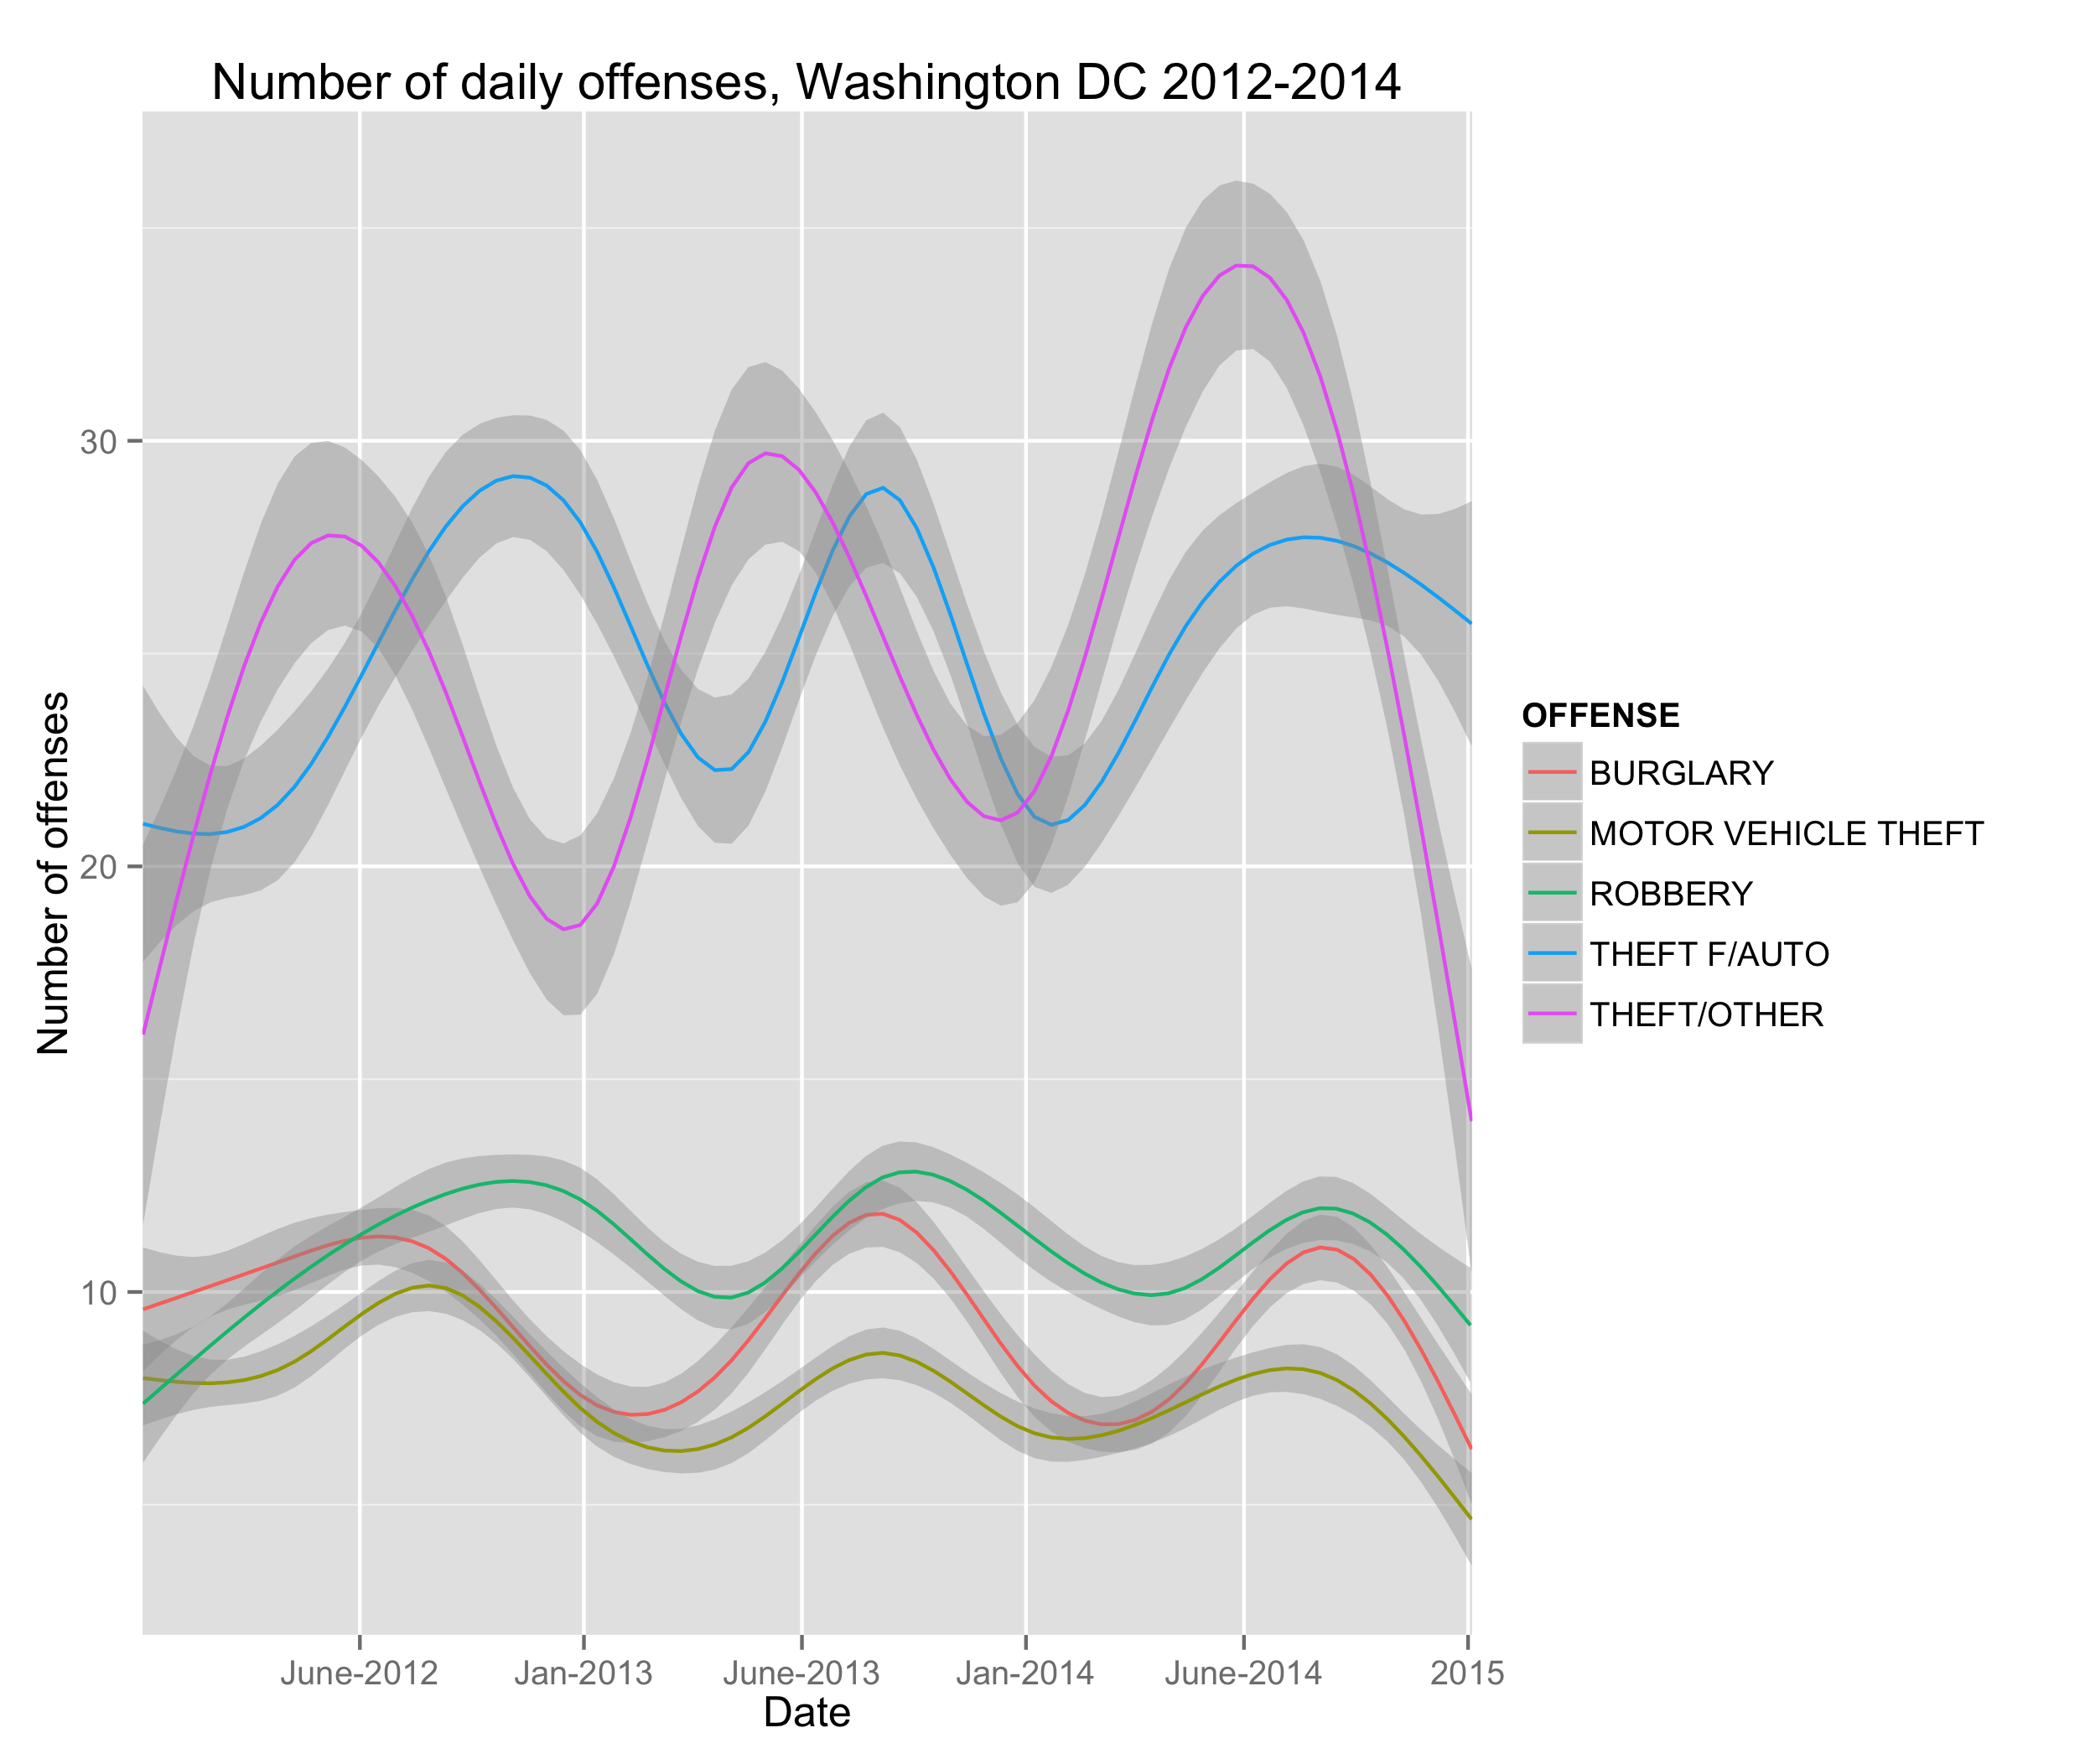
\includegraphics[viewport=5 0 800 667,clip,scale=0.27]{Figures/NumOffenses_total.png}&
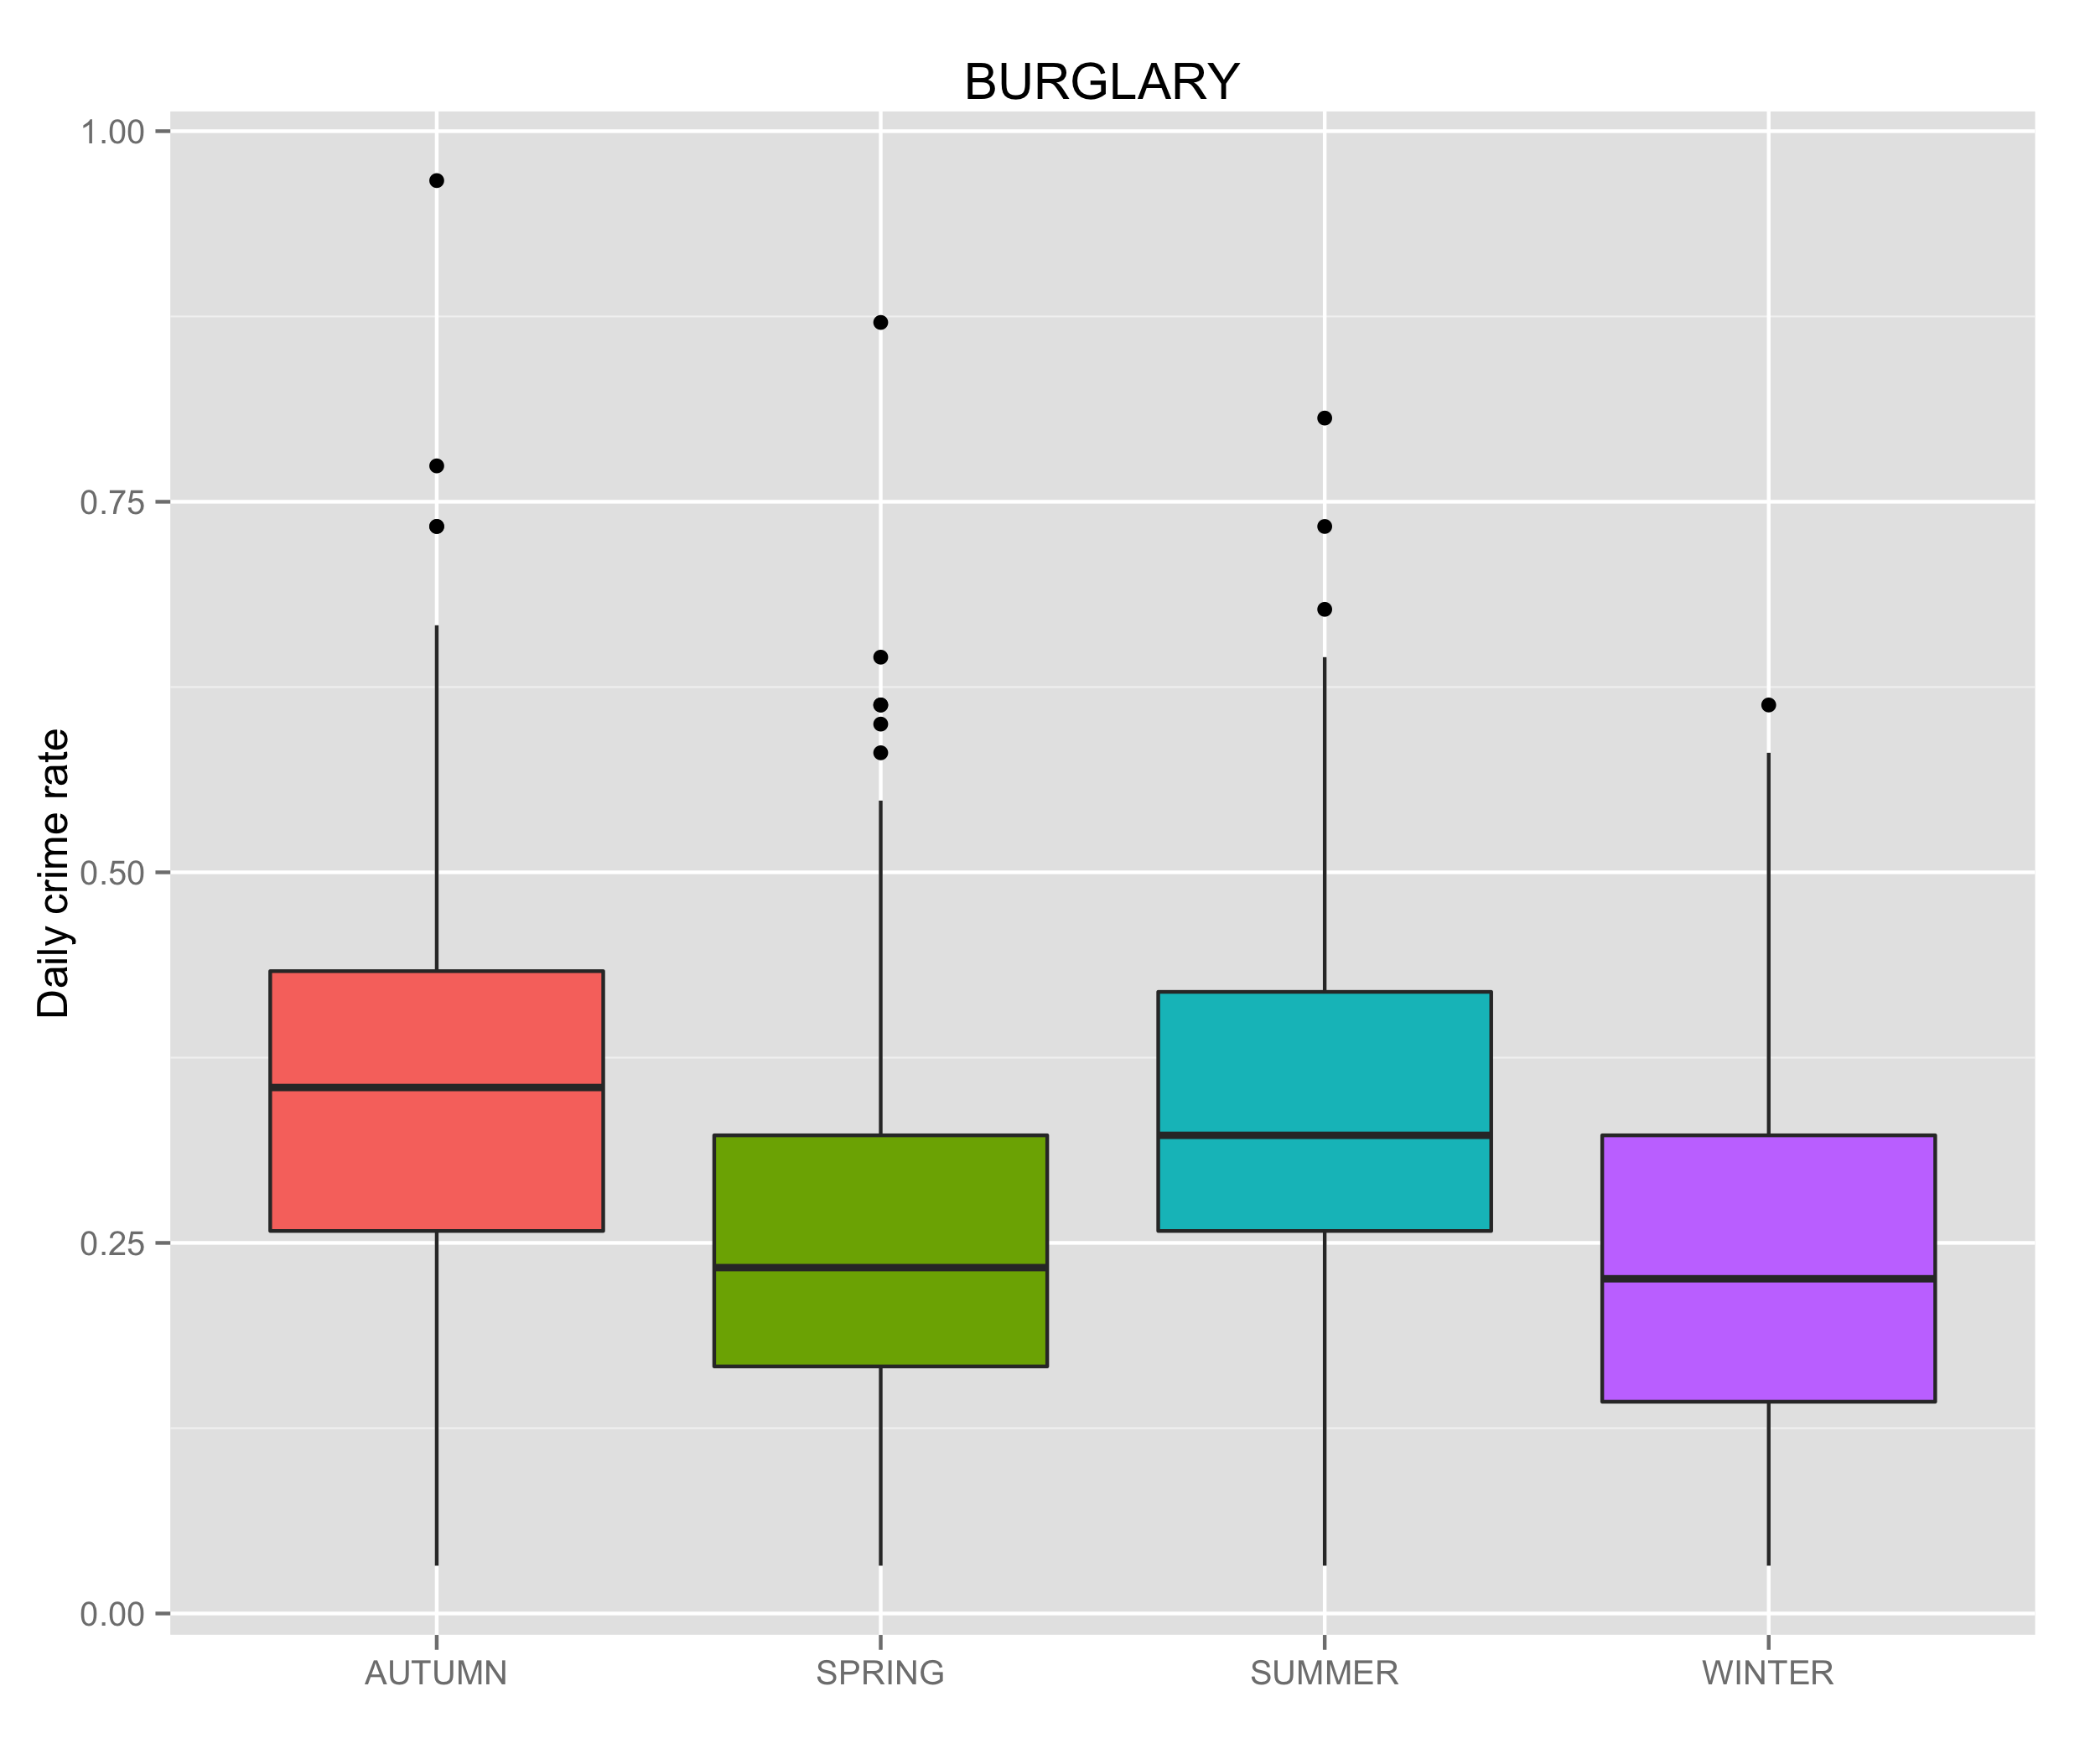
\includegraphics[viewport=20 0 800 667,clip,scale=0.27]{Figures/season_dailyRate_Burglary.png}
\end{tabular}
\caption{Seasonal variability of crime counts}\label{data}	
\scalebox{1}{
\begin{mfignotes}
The count of crime offences is clearly related to seasons.
\end{mfignotes}
}			
\end{center}
\end{figure}


%acf
\begin{figure}
\begin{center}
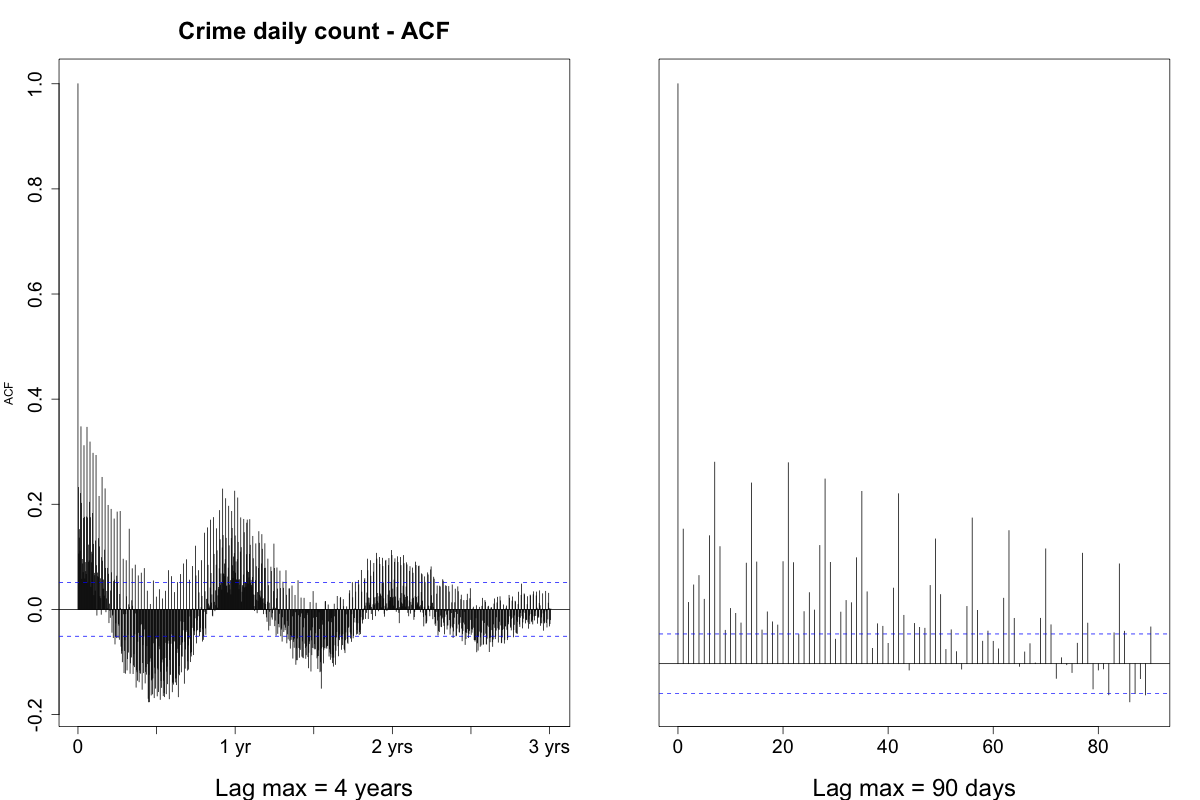
\includegraphics[viewport=0 0 1200 800,clip,scale=0.35]{Figures/ACF_crime_day.png}
\caption{Auto correlation plot: over four years and close-up over three months}\label{acf}
\scalebox{1}{
\begin{mfignotes}
The ACF shows a clear seasonal affect which diminishes over the years. A zoom into one area of the plot shows an interesting effect on the weekends.
\end{mfignotes}
}
\end{center}
\end{figure}

In this section, we will examine the temporal and spatial autocorrelation properties of the crime dataset. As we can see in Fig. \ref{data}, the count of crime offences is clearly related to seasons. In order to quantify the extent to which near observations are more similar than distant observations in time we plot the autocorrelation function (ACF) (Fig. \ref{acf}, page \pageref{acf}): values near 1 are close to perfect positive correlation and values near -1 are close to perfect negative correlation. 

At lag 0, the correlation is 1, because we are comparing the same point in time. The graph on the right in Fig. \ref{acf} shows the ACF of the daily count of offences with a lag of four years: there is a clear seasonal pattern as the positive peaks are all at the years marks. This means that every season is strongly correlated from year to year, although this correlation fades for further years. A closer view reveals also an interesting autocorrelation by the day of the week. 

%moran
\begin{figure}[h!]
\begin{center}
\begin{tabular}{cc}
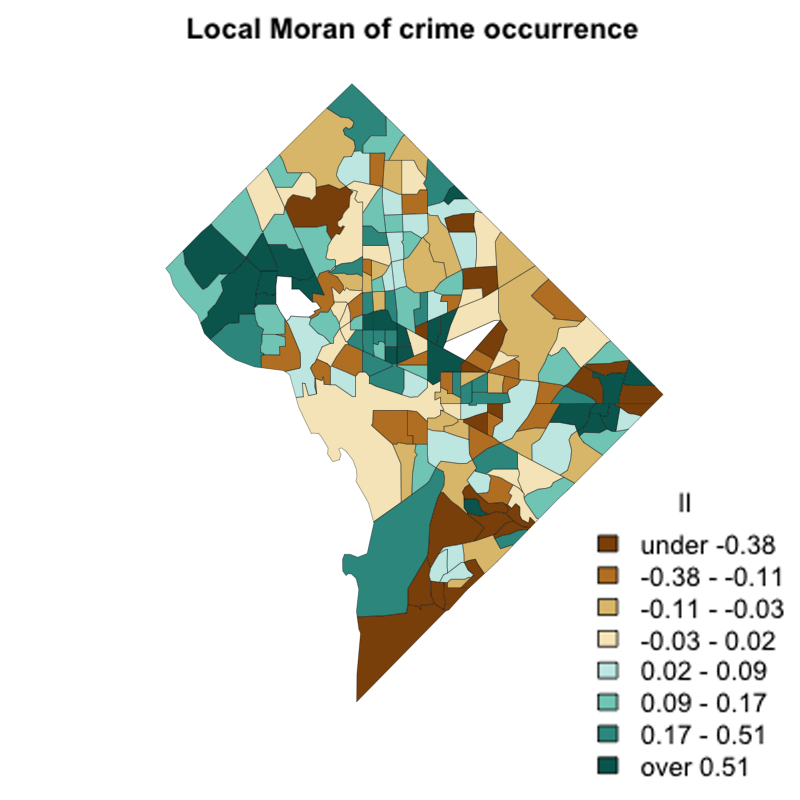
\includegraphics[viewport=5 0 800 800,clip,scale=0.27]{Figures/crimemap_LocalMoran.png}&
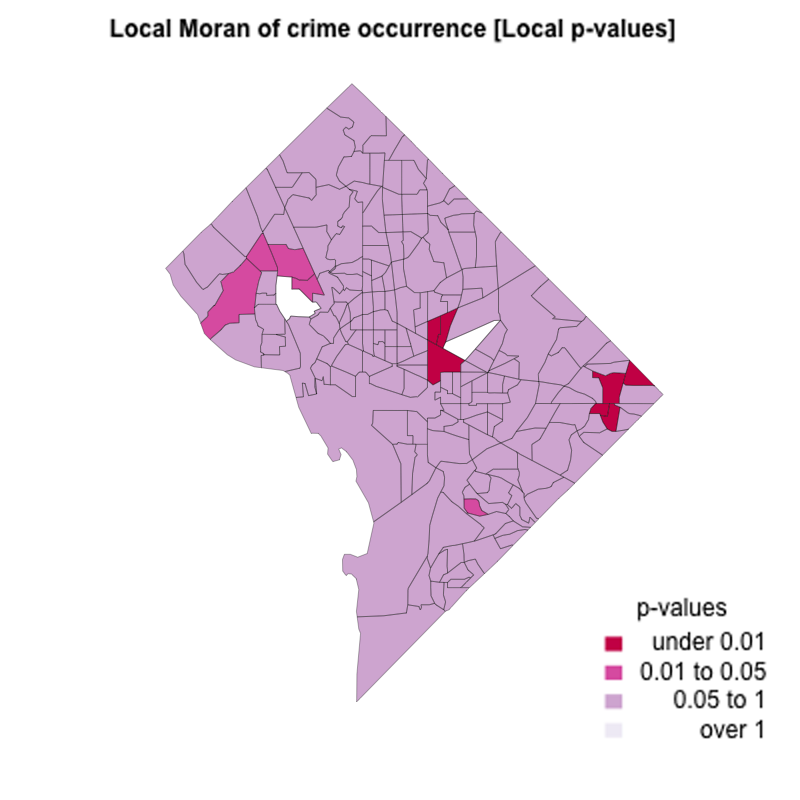
\includegraphics[viewport=20 0 800 800,clip,scale=0.27]{Figures/crimemap_LocalMoranpvalues.png}
\end{tabular}
\caption{Local Moran's I for total burglary occurrences from 2011 - 2014 and related p-values}\label{moran}
\scalebox{1}{
\begin{mfignotes}
Local Moran's I values seem to be strong in some areas, but only three areas are statistically significant.
\end{mfignotes}
}				
\end{center}
\end{figure}

The spatial correlation is less obvious: there are some areas which shows a high spatial correlation (Fig. \ref{moran}, page \pageref{moran}) but only three spots shows statistical significance. The significant areas include an affluent area near the western border containing neighbourhoods like Cleveland Park and McClean Gardens, while the significant area in the far eastern corner of the city includes a notorious chunk of neighbourhoods which have experienced high levels of violence in recent years. The significant area in the middle includes the quickly gentrifying neighbourhoods of Eckington and H Street NE.
In this experiment we will consider the aggregation of crime offences related to burglary by season, considering winter starting in December and each season during three months. 


\section{Random Forest} \label{RF}
%%%%%%%%%%%%%%%%%%%%%%%%%%%%%% RANDOM FOREST
\subsection{Overview}

\begin{figure}[h!]
\begin{center}
\begin{tabular}{cc}
\centering
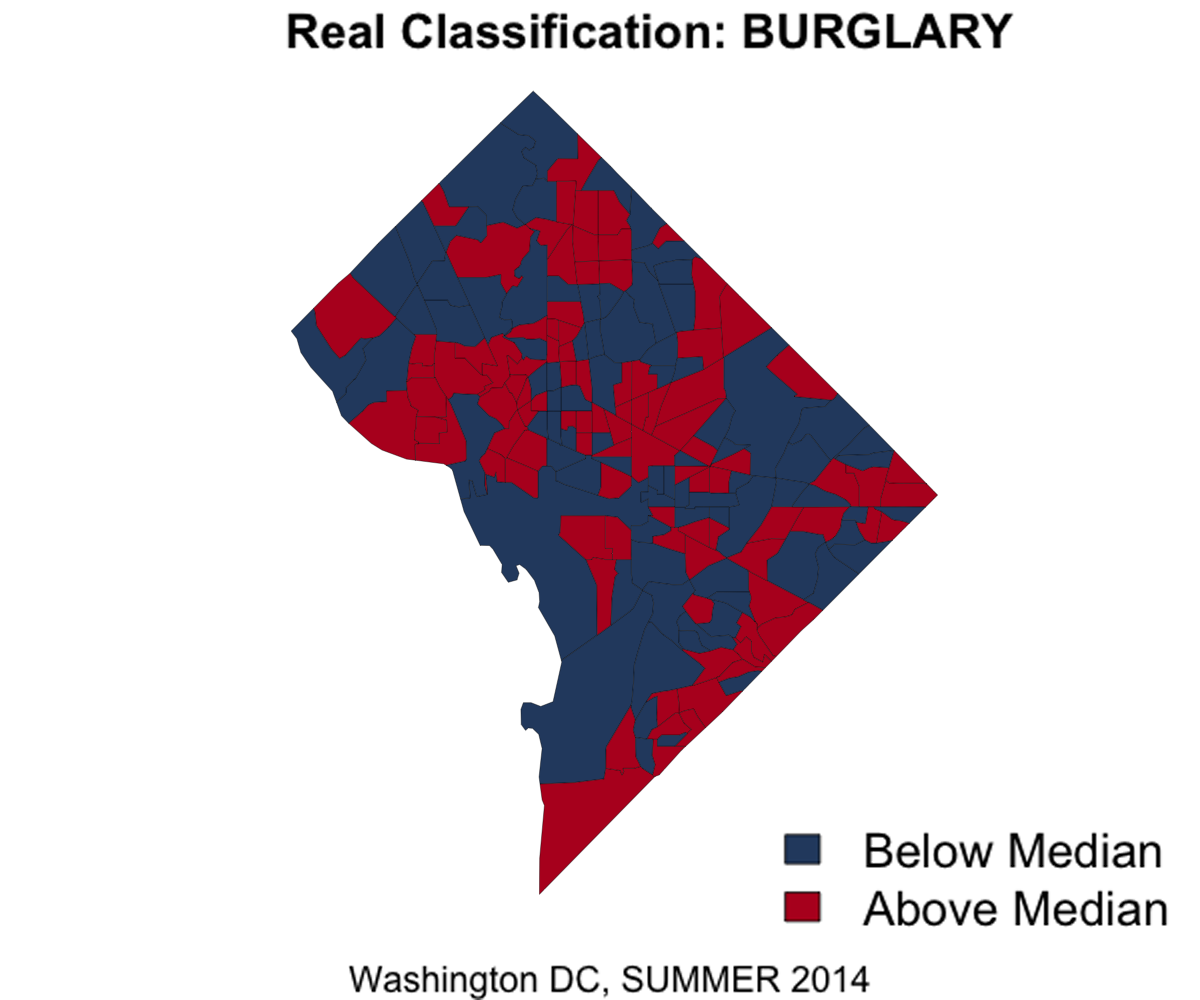
\includegraphics[viewport=260 0 1200 1000,clip,scale=0.22]{Figures/Real_classification_BURGLARY_SUMMER2014.png}&
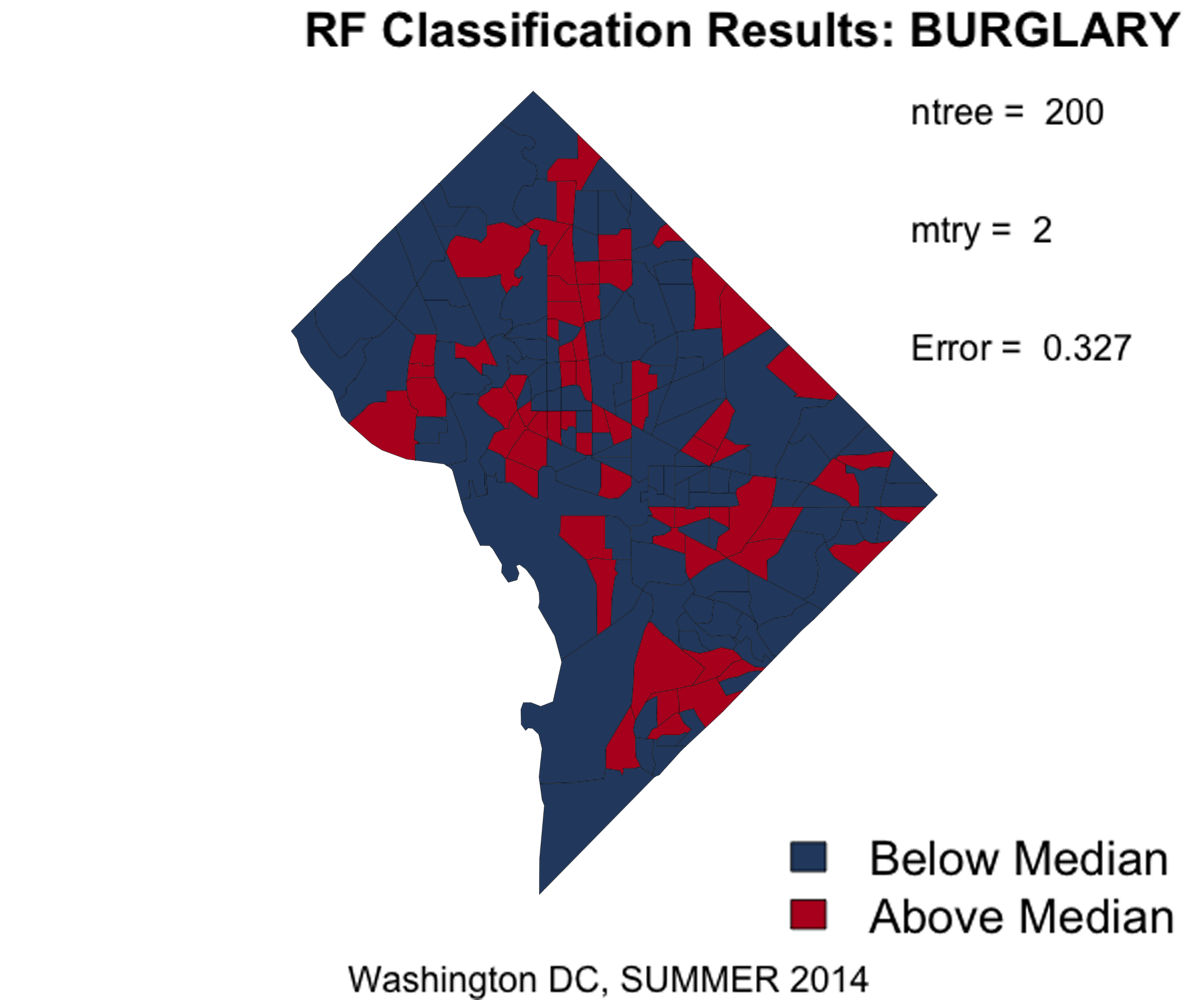
\includegraphics[viewport=260 0 1200 1000,clip,scale=0.22]{Figures/RF_prediction_BURGLARY_SUMMER2014_ntree200_2.png}
\end{tabular}
\caption{Maps of real classification vs. Random Forest prediction}\label{realClassRFmap}			\scalebox{1}{
\begin{mfignotes}
Classifies high crime areas as low crime areas more often than the opposite error.
\end{mfignotes}
}
\end{center}
\end{figure}

Random Forest, first proposed by \cite{breiman2001random}, is based on the tree classification method. In this method, many classification trees are grown, and input vectors are sent down through each tree, receiving a classification. In this way, the tree "votes" for that classification. The classification which is "voted for" by the most trees, wins. The parameters available for alteration include the number of trees (\emph{n}) to be grown, and the number variables (\emph{m}) to be used to split each node (\emph{ntree} and \emph{mtry} respectively in the randomForest package in R). At each node of the tree, \emph{m} number of variables are chosen at random from the input variables, and the best split is taken from among them at that node. The parameter \emph{m} must of course be less than the total number of variables. Two factors are shown to increase the error rate of a random forest: the correlation between trees (more correlation means higher error), and the strength of each individual tree in the forest (stronger classifiers mean lower error) \citep{breiman2001random}. While the number of trees grown does not significantly impact the error rate, decreasing the number of split values lowers both the correlation and the strength \citep{breiman2001random}. Thus, \emph{m} is the only parameter that has a significant effect on the error rate of Random Forest. Unlike in other tree classification methods, there is no pruning.

Random Forest has several advantages over other classification algorithms, including the fact that overfitting is not an issue \citep{breimancutlerRF}. It can handle thousands of input variables, runs relatively quickly, and has a high rate of accuracy relative to other methods. Of special note is the fact that it can provide estimates of which variables are most important in determining the classification output. 

\subsection{Experimental Setup}

%
\begin{wrapfigure}{R}{0.6\textwidth}
\begin{center}
\vspace{-20pt}
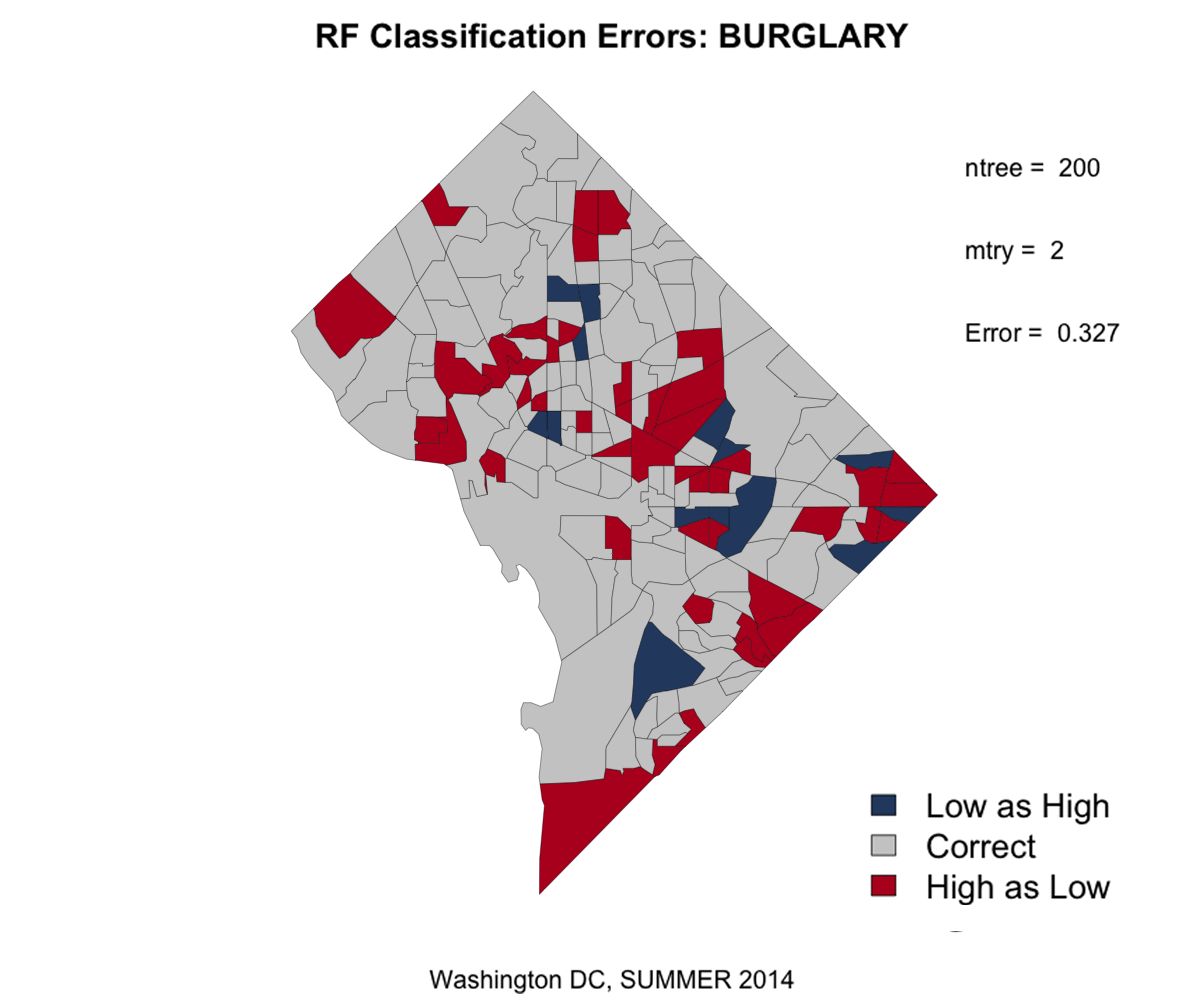
\includegraphics[viewport=200 0 1200 1000,clip,scale=0.30]{Figures/RF_errors_BURGLARY_SUMMER2014_ntree200_mtry2.png}
\caption{Classification errors with Random Forest}\label{predClassRFmap}				
\end{center}
\end{wrapfigure}

One advantage of Random Forest is that it can accept categorical variable inputs, however in order to have comparable results, we used the same initial data inputs for both SVM and Random Forest. As will be discussed in the Experimental Setup section of SVM, the seasonal variable was converted from a categorical value (SEASON = "Summer") to a binary numerical value (SUMMER = 1). We chose to focus on the crime of burglary, and so aggregated the count of incidents of burglary by year, season, and census tract. We then calculated a label for each observation, considering any value below the median of the count as a 'low" crime area, and anything above as a "high" crime area. These were labeled as -1 and 1 respectively. This formed our initial input data. 

The initial training data considered the years 2011, 2012, and 2013, with the test data being Summer 2014. We chose this time span because the demographic data from the ACS was last updated for 2014, and thus we could not test 2015. We tested against only one season at a time since the crime count was aggregated by season, and thus it makes sense for our output labels to only be applied to a single season. This is how the tool would be used to forecast police resources.

\subsection{Analysis and Results}
%var imp

\begin{wrapfigure}{R}{0.5\textwidth}
\begin{center}
\vspace{-200pt}
\centering
	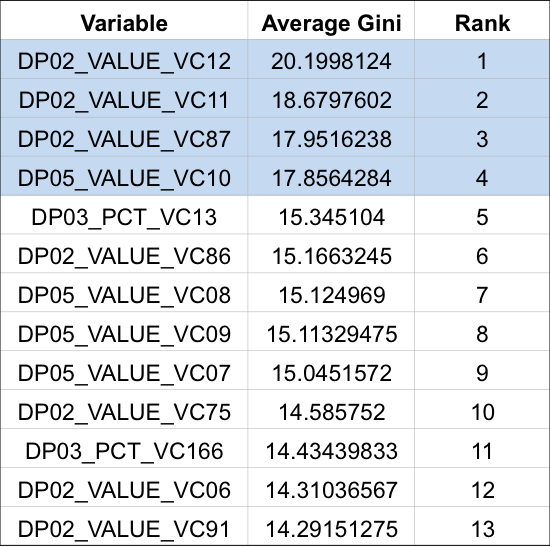
\includegraphics[viewport=-20 0 550 547,clip,scale=0.7]{Figures/varImpPlotTable.png}
\caption{Variable Importance Plot table}\label{impPlotTable}	
		
\end{center}
\end{wrapfigure}

Next I trained the model on this data using various combinations of parameters. I varied the number of trees (\emph{ntree}) between 200, 500 and 1000, and the number of split variables between 2 and 4. I ran each configuration ten times, predicted values for summer 2014, and then averaged the error. The best performing configuration of this set was \emph{ntree} = 1000, \emph{mtry} = 2 with an error rate of 31.8\%. This error rate, while the best, was not much better than other configurations that used \emph{mtry} = 2. Increasing \emph{mtry} consistently increased the error rate. This outcome is consistent with the idea that the number of trees does not have a great effect on error rate, however the model is sensitive to the number of split variables \citep{breiman2001random}. Next, I narrowed the training data to only the first year, 2011, and reran the model. The benefit of using only one year of training would be decreasing run time and general simplification. The optimal configuration for this set was \emph{ntree} = 500, \emph{mtry} = 2 with an error of 31.8\%, the same as when using all years of data.

% Imp Chart
\begin{wrapfigure}{R}{0.5\textwidth}
\begin{center}
\vspace{-290pt}
\centering
	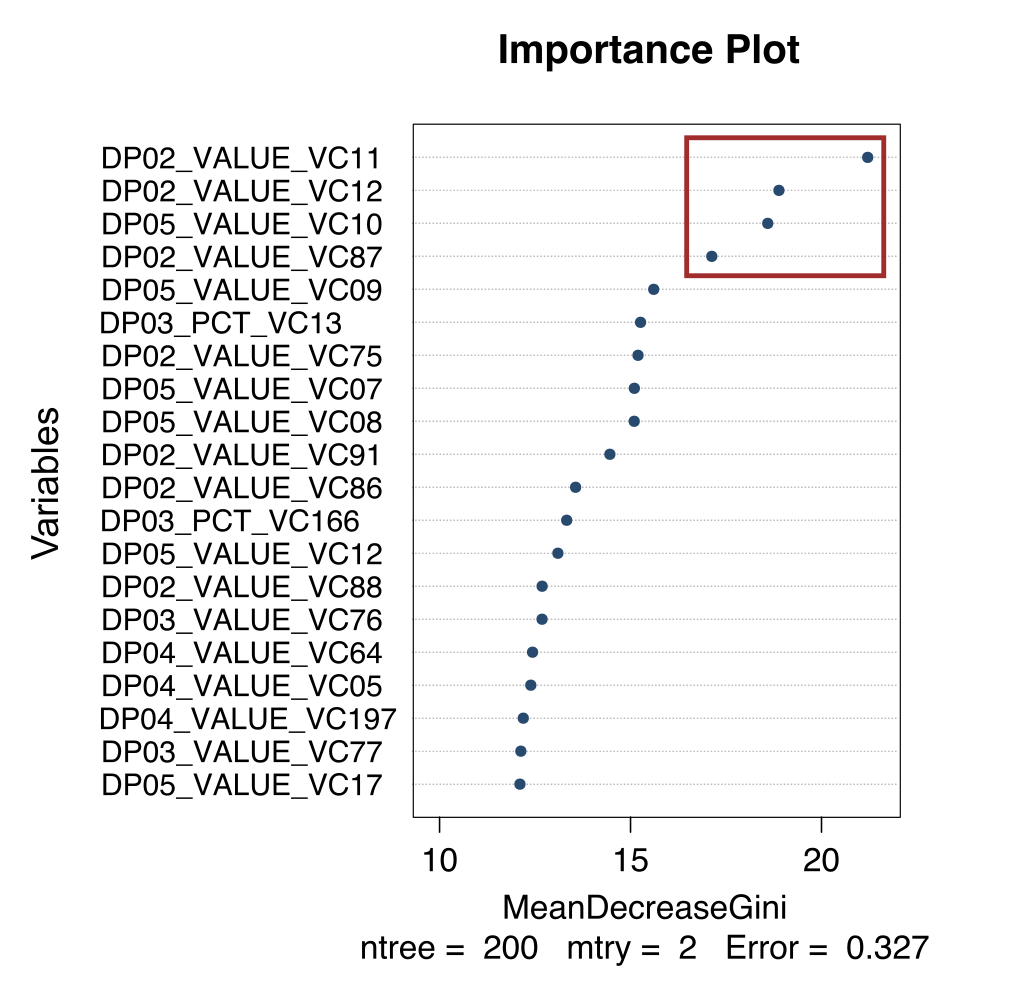
\includegraphics[viewport=0 0 1018 992,clip,scale=0.5]{Figures/varImpPlotChart.png}
\caption{Variable Importance Plot chart}\label{impPlotChart}	
\vspace{10pt}
\end{center}
\end{wrapfigure}


During the first set of configurations, I recorded the Variable Importance Plot values into a table and found the average of the values for mean decrease in node impurity (Fig. \ref{impPlotTable}, page \pageref{impPlotTable}). This tells us which variables are most important contributors to the model. This is a capability that is unique to Random Forest. The top four variables are Household Type: Female householder, no husband present, family - With own children under 18 years; Household Type: Female householder, no husband present, family; Educational Attainment: High school graduate or equivalent; and Age: 15 to 19 years old (Fig.  \ref{impPlotChart}, page \pageref{impPlotChart}).




To see how accurately a simplified model would perform, I trained the model on these four top performing variables for the years 2011 - 2013, predicted for summer 2014, and averaged the errors for the various configurations. The minimum error increased noticeably (to 37.1\%), but considering that 87\% of the variables were removed, this is actually impressive. Given that one of the benefits of machine learning is that it can handle a large amount of input variables, and that the processing time was not vastly improved, it seems reasonable to keep all of the original variables. The full set of resulting errors on each configuration can be viewed in Fig. \ref{RFerrors}.


%RF errors
\begin{figure}
\begin{center}
\centering
\vspace{-200pt}
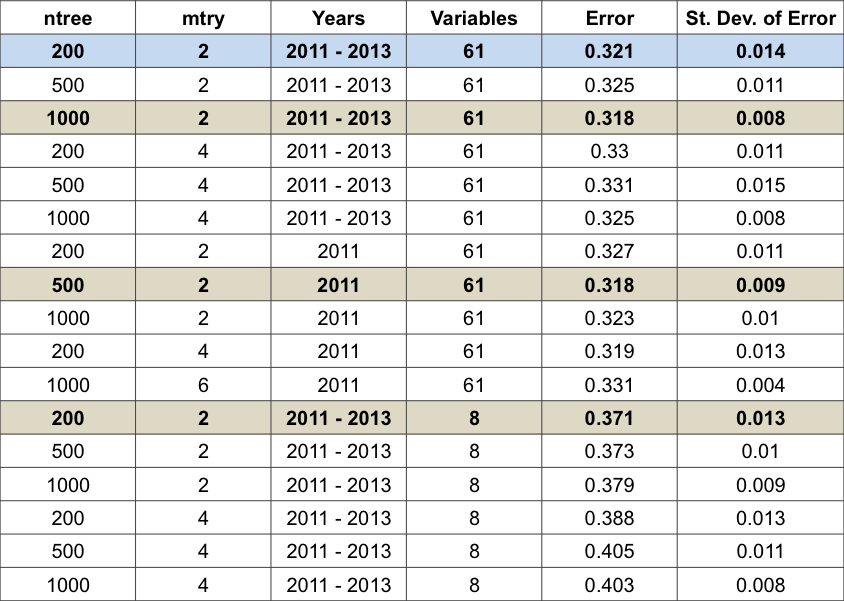
\includegraphics[viewport=-80 0 844 601,clip,scale=0.8]{Figures/RFerrors.png}
\caption{Table of error rates of tested Random Forest parameter configurations}\label{RFerrors}	\scalebox{1}{
\begin{mfignotes}
Highlighted rows indicate highest performing configuration for the given set of training data.
\end{mfignotes}
}	
\end{center}
\end{figure}

Fig. \ref{realClassRFmap} (page \pageref{realClassRFmap}) and Fig. \ref{predClassRFmap} (page \pageref{predClassRFmap}) show the results of running classification for burglary using the optimal parameters of ntree = 200, mtry = 2 on a training dataset using the years 2011 - 2013 and testing for the summer of 2014. The resulting error was 0.327 or 32.7\% on this trial. 



\section{SVM}
%%%%%%%%%%%%%%%%%%%%%%%%%%%%%% SVM
\subsection{The algorithm}
Support Vector Machines (SVM) are a set of supervised machine learning models used for classification and regression analysis. Given a set of training data with each observation assigned to a binary category, SVM builds a model which can take a new set of data and return the labelling for it. The basic version of SVM is a non-probabilistic binary linear classifier: data is labelled with one or two categories and the classification is obtained by linear separation. The input is represented in the feature space as a set of points to be divided by a clear margin which is as wide as possible. New examples are represented in the same space and labels are predicted based on which side of the margin they fall in. The maximum gap is found by finding the separating hyperplane and maximising the distance of the plane form the points that are used to define the margin (Support Vectors). The hyperplane is a subspace of one dimension less than the ambient space. This means, for example, that the hyperplane of a two dimensional space such as the cartesian axis is a line. When the margin is wide, the confidence in the model is high, when the margin is very small the confidence is low. In this case and when data is non-separable, it is possible to introduce soft margins \citep{cortes1995support}, by allowing a trade-off between the complexity of the model and the error. SVM can solve non-linear classification by mapping the input space into higher or infinite dimension space using the kernel trick \citep{boser1992training}. Kernels are weighting functions computed based on similarity-difference (objects less different have higher weights) first proposed by \cite{aizerman1964theoretical}. They are used in statistics (e.g. Kernel Density Estimation KDE for estimating the probability density function) and in spatial and temporal analysis (e.g. Spatial and Spatio Temporal KDE for modelling spatial and temporal decay). SVM can be used also for non-binary classifications using algorithms that reduce multi-class tasks to several binary problems. \\
\subsection{Analysis and Results}
% SVM results
\begin{figure}
\begin{center}
\vspace{-100pt}
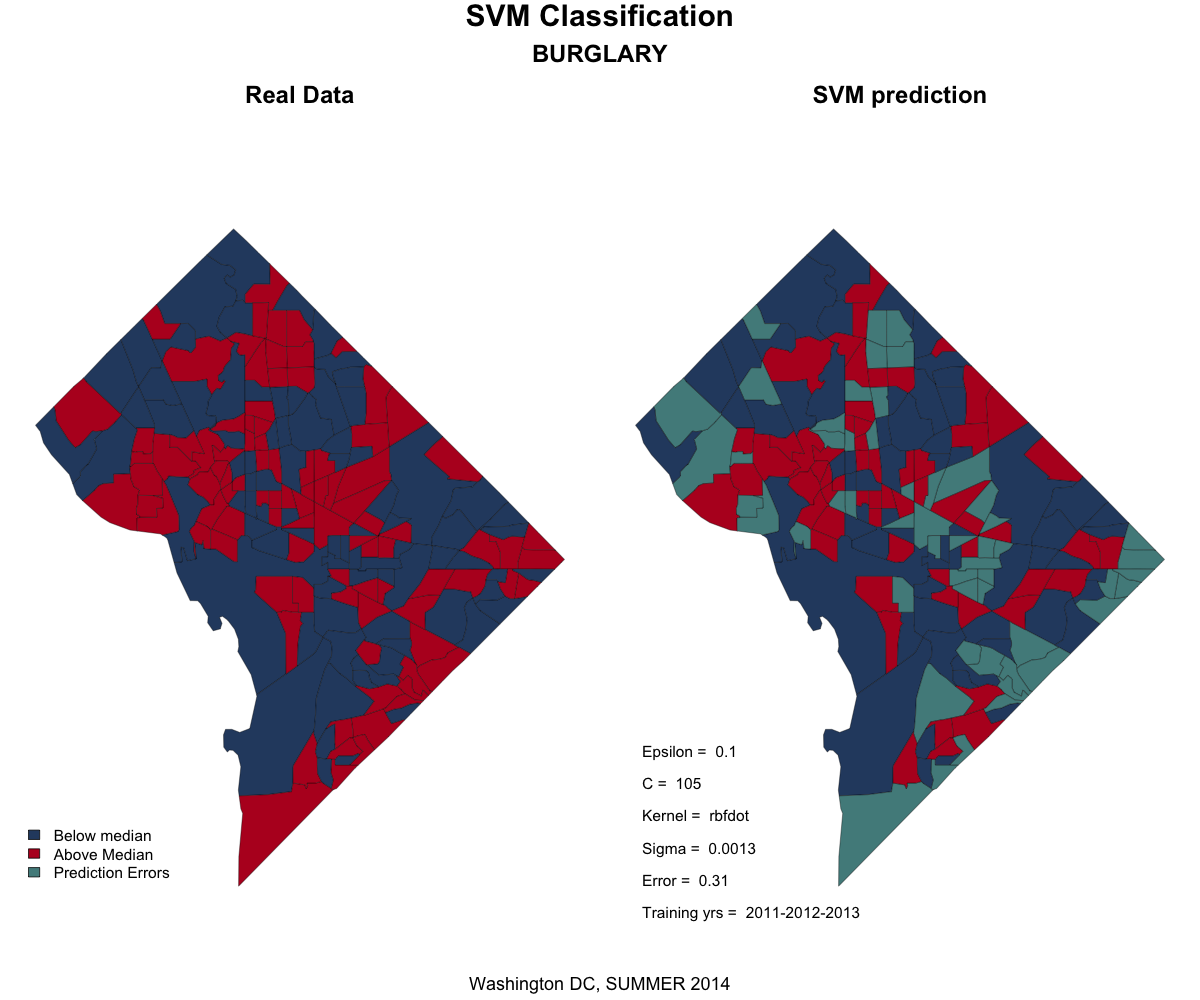
\includegraphics[viewport=0 0 1200 1000,clip,scale=0.4]{Figures/zSVM_lsM22_C105_rbfdot.png}
\caption{Prediction from the oprimized model}\label{map1M4}				
\scalebox{1}{
\begin{mfignotes}
Although not very clear, it appears that the errors lie at the borders between clusters of high crime level census tracts.
\end{mfignotes}
}
\vspace{10pt}
\end{center}
\end{figure}

  For the purpose of this essay, I will be using SVM classification methods using the Gaussian Radial Basis Function $$k(x, x\prime) = exp(-\frac{||x-x\prime||^2}{2\sigma^2})$$ as the base kernel method although I will also test the results with the polynomial method. According to \cite{svmStatSoft}, there are two classification methods, C-SVC and nu-SVM which differ in the error function that they minimise. SVM method using C-SVC is defined by the following parameters: C is the cost function, which control how much the error is penalised - hence the trade-off between complexity and prediction accuracy - and $\sigma$ is the rate of distance decay of the Gaussian kernel (high values correspond to slow decays). In order to optimise these two parameters, I will be using the \emph{caret} package in order to initialise a k-fold cross validation with \emph{k} set to 10.  The chosen set of parameters is used to train the model and the model is then tested with the data from summer 2014. For the description of the data manipulation, refer to XXXXXXXXX. \\ 
As a first test, I am interested in determining whether there is a difference in using one or more years as training set.  The accuracy of the model is highest when training on 2011 only (Table \ref{table:TAByears}, page \pageref{table:TAByears}), where using all the years perform slightly worse. Given that 2012 and 2013 also perform slightly worse than 2011, the good performance of the latter could be due to the fact that in respect to the variables used, 2011 might be a similar year to 2014. For the rest of the test, I will be using all the three years as training set.\\

\begin{table}
\begin{center}
\begin{tabular}{l*{4}{c}r}
Training Years & Accuracy & Accuracy SD \\
\hline
2011 & 0.736 & 0.029  \\
2012 & 0.716 & 0.032  \\
2013 & 0.670 & 0.020  \\
All  & 0.680 & 0.032  \\
\end{tabular}\\
\caption{Accuracy by number of years used as training set}\label{table:TAByears}
\end{center}
\end{table}


A first grid search with parameters $\sigma = 0.001, 0.01, 0.1$ and C = 10, 100, 1000 suggests that the value of $\sigma = 0.01$ and C = 10 gives the best model performance with an accuracy of 0.71. I can refine the search grid by using values around the best performers.
\begin{table}
\begin{center}
\begin{tabular}{l*{6}{c}r}
$\sigma$ Grid & C Grid & Optimal $\sigma$ & Optimal C & Accuracy & Conf Int 0.95 \\
\hline
0.001, 0.01, 0.1 & 10,100, 1000 &0.001&100& 0.721 & $\pm$0.042  \\
0.0005, 0.001, 0.0015 & 50,100,150 & 0.0015 & 100 & 0.722 & $\pm$0.050   \\
0.0012, 0.0015, 0.0018 & 80, 100, 120 & 0.0012 & 100 & 0.7202 & $\pm$0.056  \\
0.0011, 0.0012, 0.0013  & 95, 100, 105 & 0.0013 & 105 & 0.725 & $\pm$0.057  \\
\end{tabular}
\caption{Parameter optimisation}\label{table:TABsearchgrid}
\end{center}
\end{table}
\\


\begin{figure}[h!]
\begin{center}
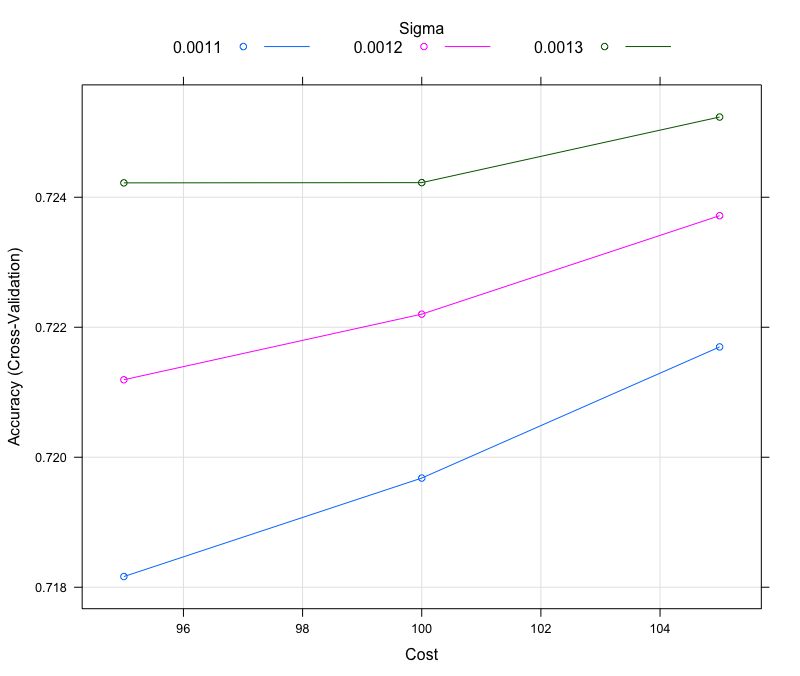
\includegraphics[viewport=0 0 800 700,clip,scale=0.35]{Figures/SVM_lsM22_ErrorPlot.png}
\caption{C plotted against accuracy by $\sigma$ values}\label{plotError}				
\scalebox{1}{
\begin{mfignotes}
In this case, for any $\sigma$, the best C value appears to be 105. Based on previous optimisation, the optimal value appears to be between 105 and 120.
\end{mfignotes}
}
\end{center}
\end{figure}

Table \ref{table:TABsearchgrid} shows different results for a sequential refinement of the parameters (see Figure \ref{plotError}): $\sigma = 0.0013$ and C = 105 give the best performance but the resulting accuracy is not statistically different from the other scenarios. The use of a higher \emph{k} for the cross validation would reduce the standard deviation and increase the precision of the search grid, but the performances are all quite similar and it would lead to no much improvement. The use of \emph{polynomial} kernel gives rather similar results in terms of accuracy, with the best accuracy performance of 0.71 achieved with degree = 2 and scale = 0.05.
In terms of time performance, all the configurations complete the training in between 25 and 35 seconds, with the exception of the polynomial kernel optimisation, which takes over an hour, without any improvement in the prediction accuracy.

%SVM support vectors
\begin{wrapfigure}{r}{0.4\textwidth}
\begin{center}
\vspace{-20pt}
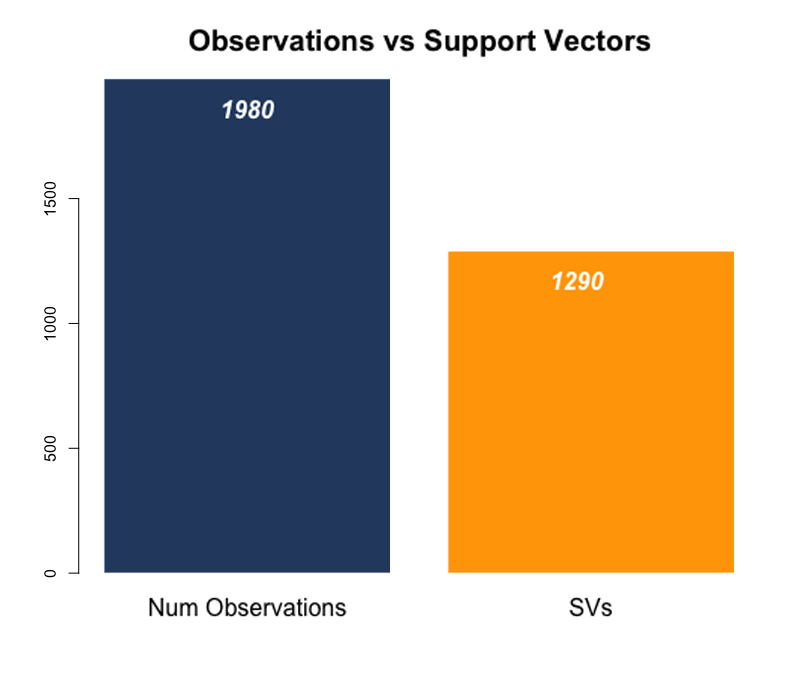
\includegraphics[viewport=25 50 800 650,clip,scale=0.26]{Figures/SVM_supportVectors.png}
\caption{Number of support vectors}\label{barplotM4}				
\end{center}
\end{wrapfigure}

An attempt at simplifying the model has been made by narrowing down the variables to the four most important in Section \ref{RF}. This slightly reduces the accuracy to about 66\%, but it also reduces the training time to about 10s in the case of the Gaussian kernel and drops it drastically in the case of the polynomial one, down to about 40s.



Figure \ref{map1M4} shows the results of the model when predicting the rate of crime in summer 2014 compared to the real data. In this example the model predicts correctly the crime level in about 30\% of the census tracts. Although this could be considered a decent prediction, the problem is that, as it is clear in Figure \ref{barplotM4}, there is a high number of support vectors. This is a clue of overfitting, which is generally addressed with the parameter optimisation as above (or more data points). In this case the problem (and the limitation of this whole exercise) might be in the data and in the little variation of the census data from one year to another. 
\clearpage




\section{Comparison}

%Comparison
\begin{figure}
\begin{center}
\centering

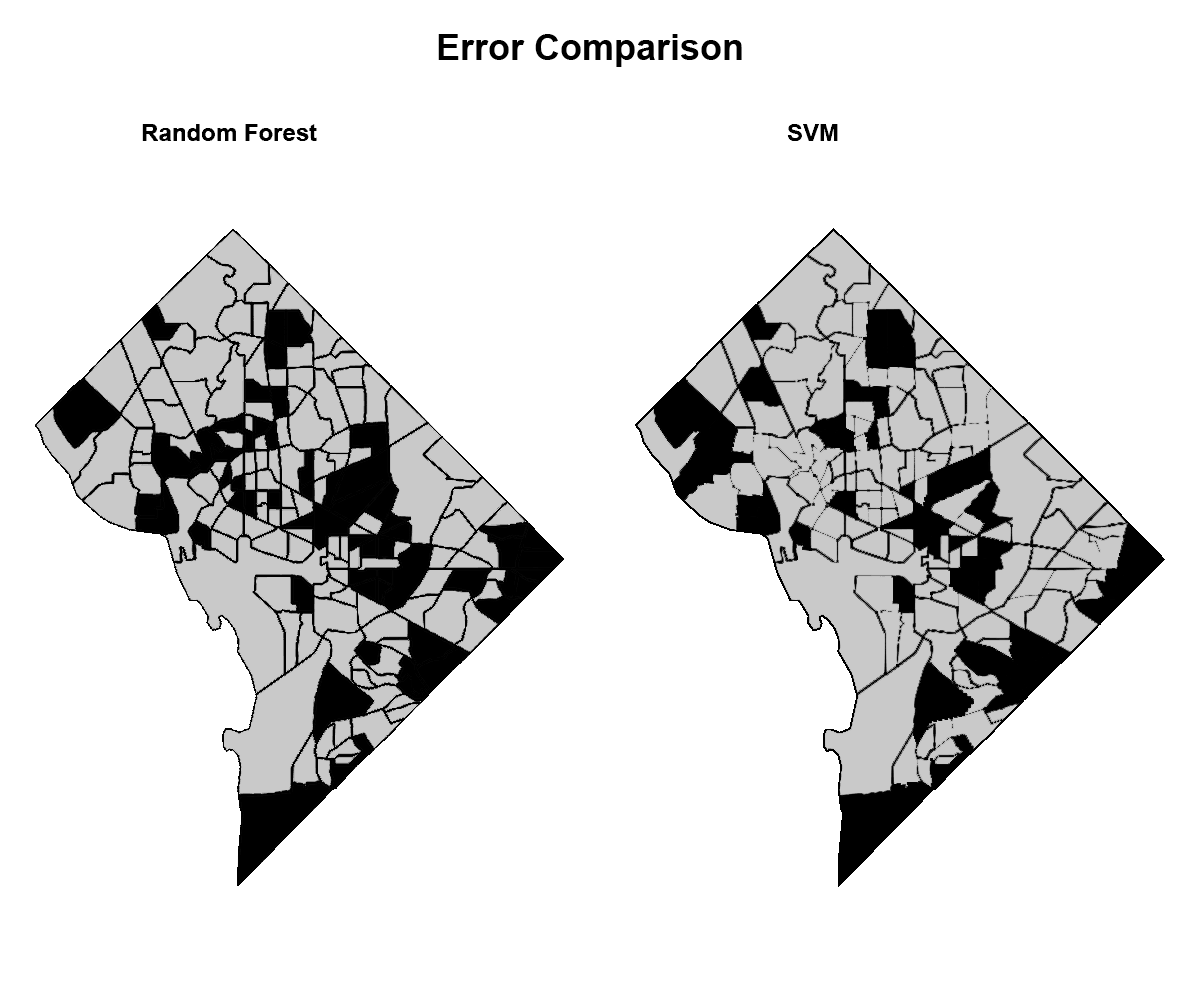
\includegraphics[viewport=0 0 1200 1000,clip,scale=0.4]{Figures/error_comparison.png}
\caption{Error comparison between RF and SVM}\label{comparisonBW}	
\scalebox{1}{
\begin{mfignotes}
In grey the census tracts correctly labeled and in black the errors.
\end{mfignotes}
}			
\end{center}
\end{figure}


\subsection{Overview}


It is generally agreed that Random Forest and SVM are amongst the best performing classifiers:  \cite{Fernandez2014we} found that they consistently perform better than all the other algorithms in a long list and, although Random Forest is ranked at the first place and SVM second, there is no statistically difference in the performances of the two.  In the present experiment, SVM performed better than Random Forest by only a small margin (Fig. \ref{comparisonBW}), about 2-3\%. This difference is quite small and it might not be statistically relevant. In Fig. \ref{overlap}, we can see how the errors are most of the time the mislabelled census tracts overlap: the two algorithm perform almost the same and with the same behaviour. Amongst the qualities of Random Forest, it is generally mentioned its simplicity of implementation and the relatively low number of parameters to be set.

%Overlap
\begin{wrapfigure}{r}{0.5\textwidth}
\begin{center}

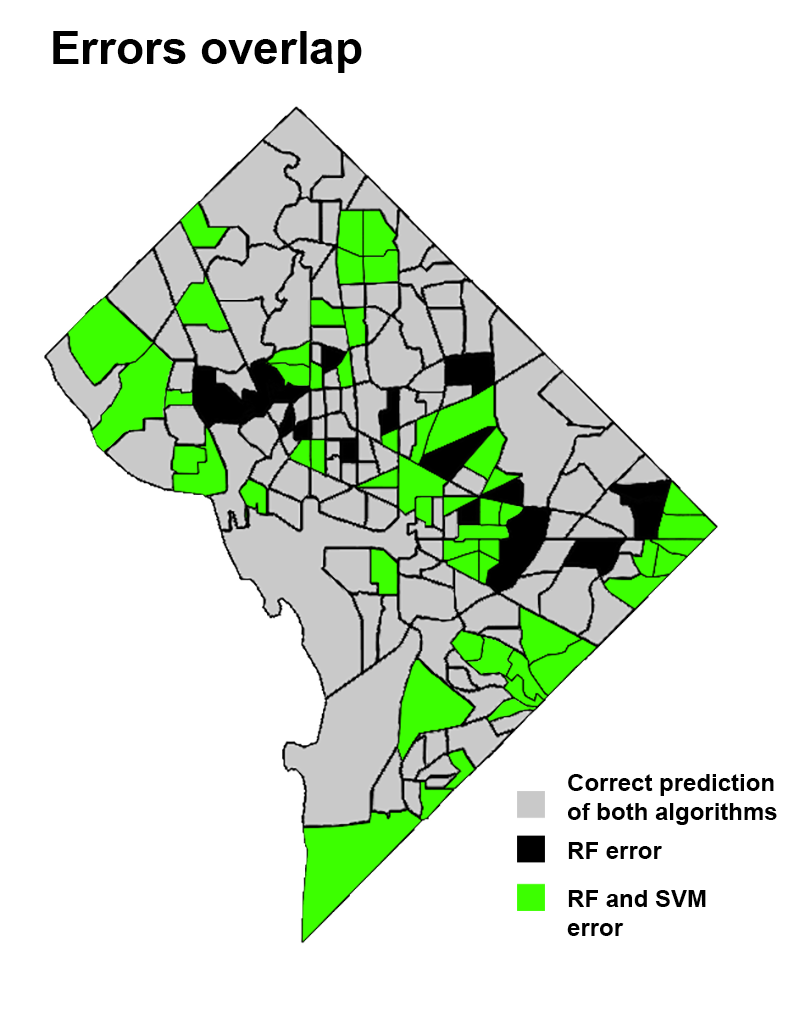
\includegraphics[viewport=0 0 800 1029,clip,scale=0.32]{Figures/error_comparison_overlap.png}
\caption{Overlap of the results.}\label{overlap}				
\end{center}
\end{wrapfigure}

 Furthermore, Random Forest can take categorical variables and it is usually a fast performer. SVM performs well when there is a high number of dimensions (it is used, for example, in text classification) and is very adaptable because it can use a vast number of kernel functions. On the other hand, this means a lot of parameters and different functions to choose from make the implementation more complex. It also requires the categorical variables to be split into multiple binary variables, which can be daunting when the categories are more than two or three. On the plus side, SVM can be used in regression analysis. 
For the purpose of this experiment, the running time turned out not to be an issue and the training time was almost always within a minute. SVM, though, needs the calibration of the parameters by means of search grid and this takes a little more time. In particular, when used with a polynomial kernel, the training time grows from few minutes to hours without much improvement in the results. Overall in the case considered here, if the accuracy of the results is the priority, SVM is the best choice. On the other hand, were simplicity and time the priorities, Random Forest would probably be a better solution.



\subsection{Limitations and further studies}

The experiment was designed at the beginning as a tool to predict crime in the short period using variables that can be monitored on a daily or hourly basis. Based on literature review and data analysis which suggest seasonality, temperature and weather conditions were considered as possible candidates. It turned out that there is little or no direct connection between crime and weather, therefore we decided to redesign the experiment to create a tool to predict crime levels on the long term for resource allocation from one year to the other. We decided to aggregate the data by seasons and this reduced the amount of training data available: as a first step to improve the model, the training data should be extended to cover more years rather than just the three used here. These would also reduce the risk of overfitting, which we suspect is at work in our case. It would also be interesting to train the data on other American cities, possibly assigning categories to census tracts about the primary and secondary activity of the area and the presence of other features such as museums, harbours, monuments, etc. 
The ACS survey contains a high number of variables; a further exploration of these variables would certainly increase the accuracy. The level of unemployment is monitored on a monthly basis and could therefore be included at a finer scale, say by season rather than yearly. Another interesting addition would be to include the level of police forces on the territory from the past years to include the interaction between crime level and police patrolling level. These would make the tool more useful, as it would create a response to the resource allocation and could be used to asses policies.
For all these improvements, probably Random Forest would be our choice because of the handling of categories, the ease of implementation and the possibility to determine the relative importance of the variables in the classification process.




\clearpage

\section{Appendix}\label{appendix}
%%%%%%%%%%%%%%%%%%%%%%%%%%%%% APPENDIX


\clearpage

\bibliographystyle{agsm}
\bibliography{STDM_references}


\end{document}